\documentclass[conference,12pt]{IEEEtran}
\usepackage{pdflscape}
\usepackage{hyperref}
\usepackage{tabularx}
\usepackage{graphicx, subfigure, amsmath} 
\usepackage{pdfpages}
\usepackage[backend=biber,style=ieee]{biblatex}
\usepackage[section]{placeins}
\addbibresource{References/References.bib}
\interdisplaylinepenalty=2500

% correct bad hyphenation here
\hyphenation{}
%DIF PREAMBLE EXTENSION ADDED BY LATEXDIFF
%DIF UNDERLINE PREAMBLE %DIF PREAMBLE
\RequirePackage[normalem]{ulem} %DIF PREAMBLE
\RequirePackage{color}\definecolor{RED}{rgb}{1,0,0}\definecolor{BLUE}{rgb}{0,0,1} %DIF PREAMBLE
\providecommand{\DIFaddtex}[1]{{\protect\color{blue}\uwave{#1}}} %DIF PREAMBLE
\providecommand{\DIFdeltex}[1]{{\protect\color{red}\sout{#1}}}                      %DIF PREAMBLE
%DIF SAFE PREAMBLE %DIF PREAMBLE
\providecommand{\DIFaddbegin}{} %DIF PREAMBLE
\providecommand{\DIFaddend}{} %DIF PREAMBLE
\providecommand{\DIFdelbegin}{} %DIF PREAMBLE
\providecommand{\DIFdelend}{} %DIF PREAMBLE
%DIF FLOATSAFE PREAMBLE %DIF PREAMBLE
\providecommand{\DIFaddFL}[1]{\DIFadd{#1}} %DIF PREAMBLE
\providecommand{\DIFdelFL}[1]{\DIFdel{#1}} %DIF PREAMBLE
\providecommand{\DIFaddbeginFL}{} %DIF PREAMBLE
\providecommand{\DIFaddendFL}{} %DIF PREAMBLE
\providecommand{\DIFdelbeginFL}{} %DIF PREAMBLE
\providecommand{\DIFdelendFL}{} %DIF PREAMBLE
%DIF END PREAMBLE EXTENSION ADDED BY LATEXDIFF
%DIF PREAMBLE EXTENSION ADDED BY LATEXDIFF
%DIF HYPERREF PREAMBLE %DIF PREAMBLE
\providecommand{\DIFadd}[1]{\texorpdfstring{\DIFaddtex{#1}}{#1}} %DIF PREAMBLE
\providecommand{\DIFdel}[1]{\texorpdfstring{\DIFdeltex{#1}}{}} %DIF PREAMBLE
%DIF END PREAMBLE EXTENSION ADDED BY LATEXDIFF

\begin{document}
%
% paper title
\title{RoboTractor: A Secure Signaling and Control System for Remote Management of Agricultural Vehicles using XMPP and REST}

\author{
\IEEEauthorblockN{Jeremy Wright}
\IEEEauthorblockA{Arizona State University\\jlwrigh1@asu.edu}
\and
\IEEEauthorblockN{Arun Balaji Buduru}
\IEEEauthorblockA{Arizona State University\\abuduru@asu.edu}
\and
\IEEEauthorblockN{David Lucero}
\IEEEauthorblockA{Arizona State University\\dwlucero@asu.edu}
}
\maketitle


\begin{abstract}
The need for the automation of vehicles is increasing requiring improved efficiency, operation, and reduced operational costs. The scope of this project is to build a signaling and control system \DIFaddbegin \DIFadd{for automation of vehicles, }\DIFaddend with a focus on security \DIFdelbegin \DIFdel{, in order to drastically reduce }\DIFdelend \DIFaddbegin \DIFadd{to make the systems safer by drastically mitigating the risks of }\DIFaddend the systems from being compromised. An attack against these systems could allow for the vehicles to be stolen, damaged, hijacked, or cause other losses. The main tasks in this project are to build a secure front-end web interface for users to give instructions \DIFdelbegin \DIFdel{, }\DIFdelend \DIFaddbegin \DIFadd{and view vehicle status -- }\DIFaddend built upon a Representational State Transfer (REST) architecture, set up an Extensible Messaging and Presence Protocol (XMPP) server and client with required authentication, data integrity check mechanisms and encryption, and build a simulated automated vehicle \DIFdelbegin \DIFdel{, }\DIFdelend \DIFaddbegin \DIFadd{with simulated Trusted Platform Module (TPM) similar to what would be used to secure a real vehicle, and to enable the simulated vehicle to be }\DIFaddend capable of interfacing with the XMPP components and front-end. 
\end{abstract}

\begin{IEEEkeywords}
    Secure \DIFdelbegin \DIFdel{signaling and control, remote management, agricultural vehicles
    automation, self-driven vehicles}\DIFdelend \DIFaddbegin \DIFadd{Signaling and Control, Remote Management, Vehicle Automation, Self-Driven Vehicles}\DIFaddend , TPM, \DIFdelbegin \DIFdel{root of trust, trusted platform}\DIFdelend \DIFaddbegin \DIFadd{Root of Trust, Trusted Platform}\DIFaddend , TrustZone, ARM, \DIFdelbegin \DIFdel{machine automation
}\DIFdelend \DIFaddbegin \DIFadd{Machine Automation, XMPP, Rest, RESTful methodology, Simulation, Framework, Cryptography
}\DIFaddend \end{IEEEkeywords}

\section{Introduction}
\IEEEPARstart{A}{griculture} has a growing problem. Crop input costs such as water,
fertilizer, pesticides, and fuel, are increasing. The global population is
increasing\DIFaddbegin \DIFadd{, }\DIFaddend driving the need for more food. Local, State, and Federal governments
are increasing oversight and reporting requirements on growers. Land area
available for planting, and harvesting is decreasing globally. All this pushes
farmers to rely on technology to improve their efficiency while reducing
recurrent costs. Take government oversight requirements
\autocite{_growers_oversight}, growers are required to track where, and how much
material is spread into the fields.  This can be a considerable overhead for
growers, however an automated machine can do this quite easily, and in real-time
if desired.  This project demonstrates how to securely connect an agricultural
machine to an automation server in a secure manner using existing internet
technologies. Using existing technologies is a critical point. The market is
already stretched thin, and incurring new infrastructure in rural areas can be
prohibitively expensive, however leveraging the existing Internet infrastructure\DIFaddbegin \DIFadd{, }\DIFaddend we
can provide high levels of service in a secure manner.

The most important requirement in developing a secure signal and control system is ensuring authentication of vehicles and data integrity, and securing communication channels. The path plan and location feedback transmission needs to be secured and protected from eavesdroppers, preventing attackers from compromising and/or stealing these vehicles. In this project we use the Django web framework to handle the front end interface and server duties. Django facilitates the use of python libraries and components to interface between our Front-end, server, and client-side vehicle simulators. The \DIFdelbegin \DIFdel{end-goal }\DIFdelend \DIFaddbegin \DIFadd{end goal }\DIFaddend of RoboTractor is to have a comprehensive tool that translates the abstract user inputs into remotely executable actions for agricultural vehicles in a secure manner using advanced web, network, and cryptographic techniques.

RoboTractor is a framework to provide integrity, authentication, and root of
trust services for machine automation specifically within an agriculture domain.
Electronic Control Unit (ECU) manufacturers will particularly be interested in the root-of-trust details
described in Section~\ref{sec:xmpp}.  Agricultural service providers have
typically \DIFdelbegin \DIFdel{be }\DIFdelend \DIFaddbegin \DIFadd{been }\DIFaddend subject to locality issues. Historically, it's been difficult to
provide agricultural services at a reasonable cost, at any appreciable distance
from the farm itself.  RoboTractor provides a conduit for service providers to
provide their services at a distance. This allows expert agronomists to consult
with farms at any distance.  Not only can this reduce cost, but it also allows
growers access to a marketplace of services before unavailable to them.
RoboTractor is the foundation for connecting the needs of the growers to the
providers.  

\section{System Models}

\subsection{System Model}
RoboTractor \DIFdelbegin \DIFdel{will leverage }\DIFdelend \DIFaddbegin \DIFadd{leverages }\DIFaddend the Django Web framework \autocite{_django_2014}
\DIFdelbegin \DIFdel{, }\DIFdelend to realize the required interfaces. Figure~\ref{fig:softwarecomponents} describes the connection of
these components.  The combination of XMPP and REST in RoboTractor is
a demonstration of how to extend the existing HTTP development environment
i.e. \DIFdelbegin \DIFdel{"}\DIFdelend \DIFaddbegin \DIFadd{``}\DIFaddend the web of things\DIFdelbegin \DIFdel{" }\DIFdelend \DIFaddbegin \DIFadd{'' }\DIFaddend into a stateful protocol. HTTP is by design
stateless. XMPP on the other hand is a stateful streaming connection between two
clients. In this case the \DIFdelbegin \DIFdel{Tractor }\DIFdelend \DIFaddbegin \DIFadd{vehicle (tractor simulation) }\DIFaddend and a command server.  To achieve this mesh we
will leverage \DIFdelbegin \DIFdel{the Bidirectional-streams Over Synchronous HTTP standard
protocol }%DIFDELCMD < \autocite{paterson_bidirectional-streams_2010}%%%
\DIFdel{. BOSH provides
a standard mechanism to operate }\DIFdelend \DIFaddbegin \DIFadd{a custom XMPP script to bridge gap between Django's RESTful
interface and }\DIFaddend the streaming XMPP protocol \DIFdelbegin \DIFdel{efficiently over an
}\DIFdelend \DIFaddbegin \DIFadd{securely and efficiently over a secure
}\DIFaddend HTTP connection. This is essential for a scalable \DIFdelbegin \DIFdel{webservice.
}\DIFdelend \DIFaddbegin \DIFadd{web service.
}

\DIFaddend \subsection{Software} 
\DIFaddbegin 

\DIFaddend \subsubsection{XMPP Server} 
\DIFaddbegin 

\DIFadd{XMPP stands for Extensible
Messaging and Presence Protocol. XMPP is a communication protocol that relies
upon XML (Extensible Markup Language) for operation. XMPP is an open standard
that operates with a client-server architecture. Anyone may design, build, or
operate their own server and/or client, and be able to communicate with others
operating under the open standard. This means that XMPP is strongly
decentralized, with no master or control servers.  Additionally, XMPP has
support for security protocols such as TLS built into its base specification.
XMPP operates by opening an XML document or session between two peers. Within
this session, xml stanzas can be sent containing information.  }\DIFaddend RoboTractor uses
the ejabberd \autocite{_ejabberd} XMPP server as it provides an existing Python
interface, to integrate with the rest of our Python based ecosystem. \DIFaddbegin \DIFadd{The vehicle
simulators themselves use the open source SleekXMPP Python XMPP library as the
client side XMPP interface. This allows communication between the vehicle
simulators and the ejabberd XMPP server.  
}

\DIFaddend \subsubsection{REST Interface}
\DIFdelbegin \DIFdel{TastyPie provides REST }%DIFDELCMD < \autocite{_toastdriven/django-tastypie_2014} %%%
\DIFdel{by extending
the existing Django Models.
}\subsubsection{\DIFdel{BOSH Interchange}}
%DIFAUXCMD
\addtocounter{subsubsection}{-1}%DIFAUXCMD
\DIFdel{Punjab is an Django plugin implementation of BOSH
}%DIFDELCMD < \autocite{_twonds/punjab_2014}%%%
\DIFdel{. In addition to BOSH, this library combines
the ejabberd Users with Django Users to provide a single authentication and authorization framework. While this demo projectwill have a single user type, this
combination is critical to maintain proper use management and least-privilege authorization}\DIFdelend \DIFaddbegin \DIFadd{REST is a web idiom which stands for REpresentational State Transfer.
REST allows a website to expose data via a set of URLs. In this way REST
provides a common interface to any HTTP enabled client. As HTTP becomes more and
more pervasive REST allows one to aggregate several data sources with simple
tools. Robotractor leverages the TastyPie framework to expose the Django models
via an idiomatic REST interface }\autocite{_toastdriven/django-tastypie_2014}\DIFadd{. To
demonstrate the REST interaction with XMPP, Robotractor uses AJAX (Asynchronous
Javascript And XML) queries to interact with the data. This has the added
benefit of making the site more responsive without requiring page refreshes to
see new data. Essentially, the REST interface POSTs commands to the database.
The database acts as a queue holding the messages until the XMPP adapter is
ready to deliver them to tractor simulator.
}

\subsubsection{\DIFadd{Vehicle Simulator}} \DIFadd{The Vehicle
Simulator is the device or machinery that is meant to be the recipient of the
secure command controls and signals. For the RoboTractor project, this
simulation is entirely custom built in Python. The Simulator operates on a state
machine principle, with states for receiving data, operating on data, uploading
data, and rest and shutdown. The vehicle simulator is designed to be extensible
and easy to modify, with tunable parameters for the vehicle}\DIFaddend .

\begin{figure}
\centering
\DIFdelbeginFL %DIFDELCMD < 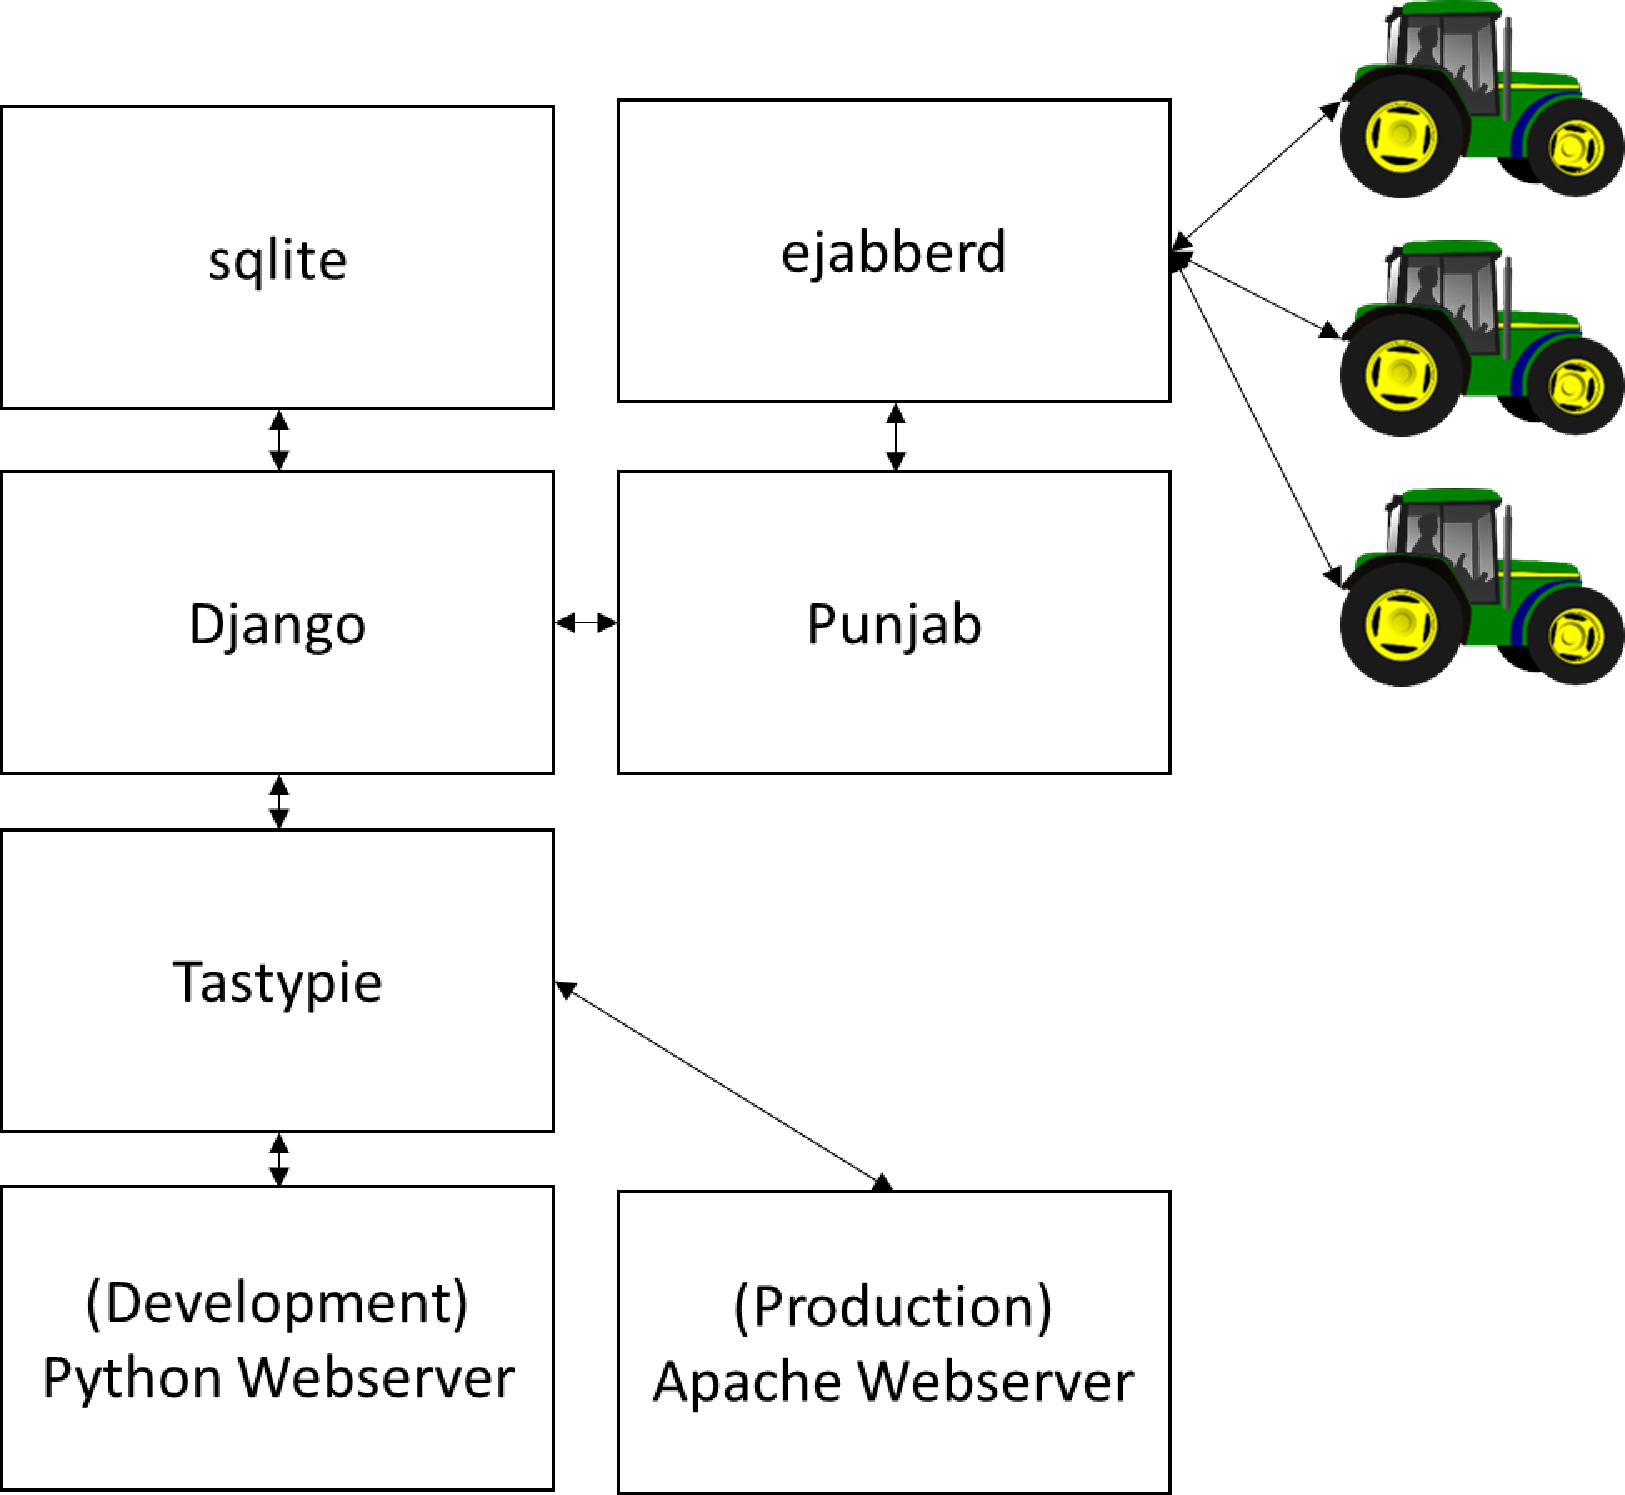
\includegraphics[width=0.4\textwidth]{SoftwareComponentBlockDiagram.pdf}
%DIFDELCMD < %%%
\DIFdelendFL \DIFaddbeginFL 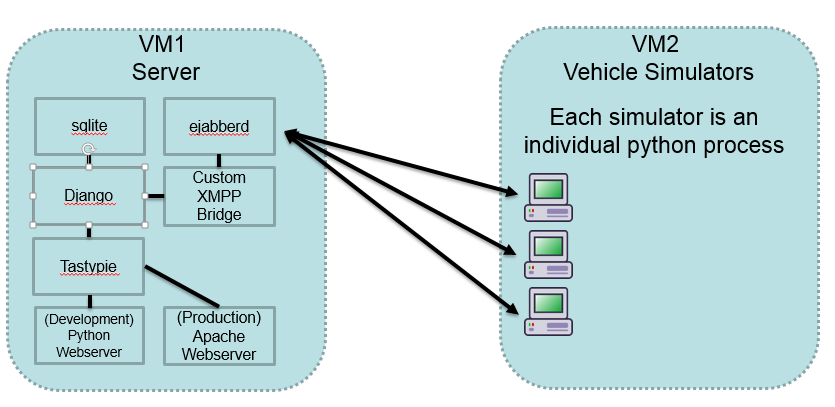
\includegraphics[width=0.5\textwidth, scale=0.5]{Images/SoftwareComponentBlockDiagram.png}
\DIFaddendFL \caption{Software Component Block Diagram}
\label{fig:softwarecomponents}
\end{figure}

\subsection{Security Model}
RoboTractor deals with two primary security classes: One involving the vehicles
and other assets, and one involving the system components and their
communication channels.  Because the project is web-based and uses PKI, numerous
attack models have been created that this project will deal with. Within the
class of communication channels, attacks may be present against the
authentication systems of both users and assets. Robotractor currently employs
advanced two-factor authentication. Usage of TLS and other best common practices
will be implemented to prevent against replay attacks on the system, and also
for establishing a secure session between assets and control. A dual-encryption
scheme has been \DIFdelbegin \DIFdel{devised }\DIFdelend \DIFaddbegin \DIFadd{used }\DIFaddend to send encrypted control signals within an encrypted XMPP
stanza to ensure high information assurance. Because this project \DIFdelbegin \DIFdel{will utilize PKI}\DIFdelend \DIFaddbegin \DIFadd{utilizes
Public Key Infrastructure}\DIFaddend , key protection is important.  To this end the
RoboTractor project \DIFdelbegin \DIFdel{plans to }\DIFdelend \DIFaddbegin \DIFadd{uses }\DIFaddend secure keys on assets with a Trusted Platform Module\DIFdelbegin \DIFdel{or relevant simulated facsimile}\DIFdelend .
By making both key-pairs private and secure, RoboTractor provides advanced
communication security. On the other end, the server components must be secured
as well using best common practices in server defense, firewall, patches,
updates, etc. Additionally, the RoboTractor system will implement an advanced
GPS location reporting system to provide physical security in case of asset
theft. By defending against these attack models, the RoboTractor project
presents the realization of an advanced system for signaling and control with
high security.

\section{Project Description}
\label{sec:proj_desc}
Implementation is divided into 2 primary phases (Marked as milestones on the
attached Gantt chart). \DIFdelbegin \DIFdel{The first phase is an integration phase connecting
}\DIFdelend \DIFaddbegin \DIFadd{In the first integration phase we connected }\DIFaddend the various
libraries and off the shelf components. \DIFdelbegin \DIFdel{It is critical }\DIFdelend \DIFaddbegin \DIFadd{We made sure }\DIFaddend that this integration \DIFdelbegin \DIFdel{does }\DIFdelend \DIFaddbegin \DIFadd{did
}\DIFaddend not weaken, but rather \DIFdelbegin \DIFdel{strengthens }\DIFdelend \DIFaddbegin \DIFadd{strengthened }\DIFaddend the security properties provided by each
independent component.

\DIFdelbegin %DIFDELCMD < \begin{figure}
%DIFDELCMD < \centering
%DIFDELCMD < 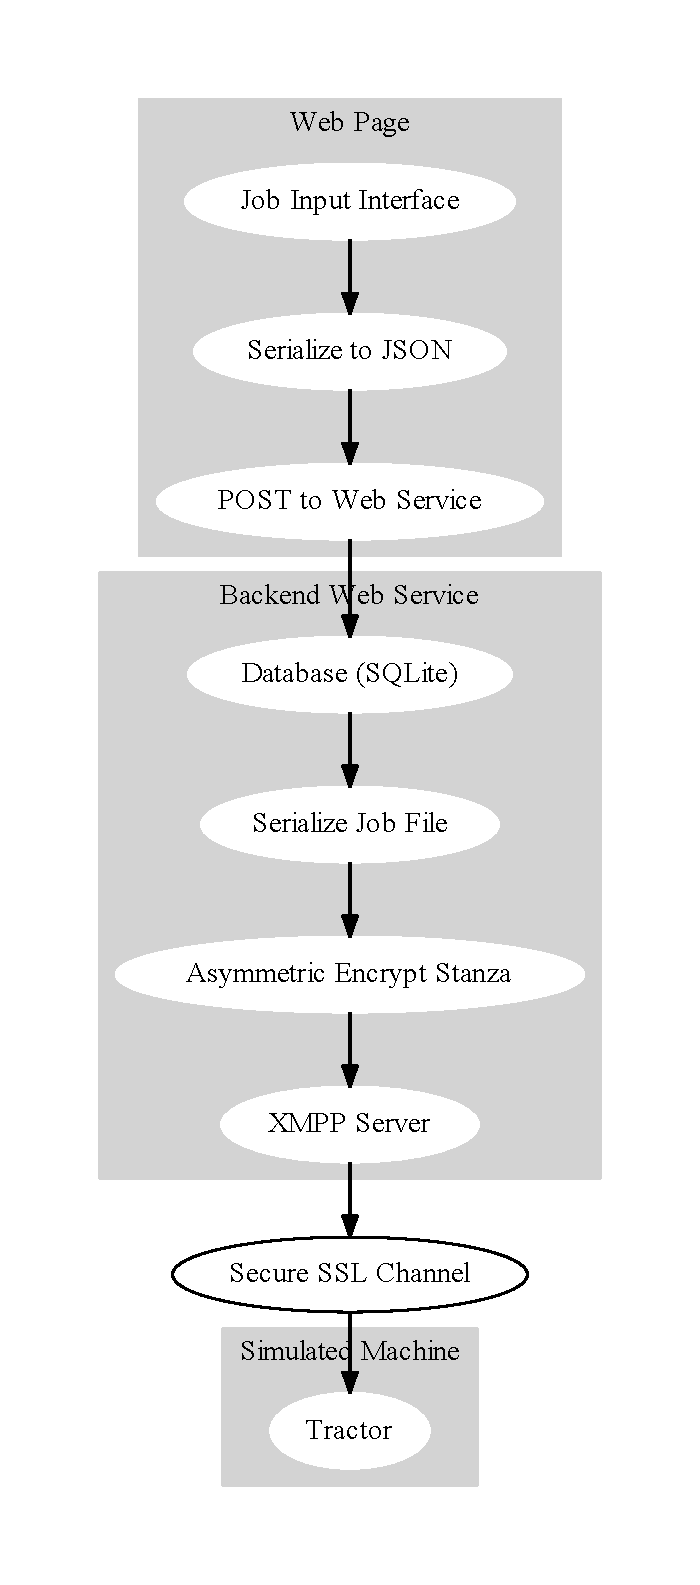
\includegraphics[width=0.4\textwidth]{signalpath.pdf}
%DIFDELCMD < %%%
%DIFDELCMD < \caption{%
{%DIFAUXCMD
\DIFdel{High Level Signal Path}}
%DIFAUXCMD
%DIFDELCMD < \label{fig:signalpath}
%DIFDELCMD < \end{figure}
%DIFDELCMD < 

%DIFDELCMD < %%%
\DIFdel{The second phase is the extension of }\DIFdelend \DIFaddbegin \DIFadd{In the second phase we extended }\DIFaddend these components to provide command and control
of agricultural vehicles. For schedule mitigation, David and Arun \DIFdelbegin \DIFdel{are
scheduled to begin }\DIFdelend \DIFaddbegin \DIFadd{completed }\DIFaddend this
phase before the framework is assembled. Once the framework \DIFdelbegin \DIFdel{is }\DIFdelend \DIFaddbegin \DIFadd{was }\DIFaddend in place, David
and Arun's interface designs \DIFdelbegin \DIFdel{may be }\DIFdelend \DIFaddbegin \DIFadd{were }\DIFaddend merged with the overall system. \DIFaddbegin \DIFadd{After this
merging, development switched focus to testing and bug fixing, since the main
components were operating at satisfactory levels. This also allowed refinement
of the front-end interface to better suit the needs of both the project, and the
rest of the RoboTractor components. }\DIFaddend As of the creation of this document, all
Midterm \DIFaddbegin \DIFadd{and Final }\DIFaddend deliverables have been achieved. The following tasks have been
updated to reflect work \DIFdelbegin \DIFdel{currently }\DIFdelend done, and remaining future \DIFdelbegin \DIFdel{work}\DIFdelend \DIFaddbegin \DIFadd{improvements that are beyond
the scope of this project}\DIFaddend .

\DIFaddbegin \begin{figure}
\centering
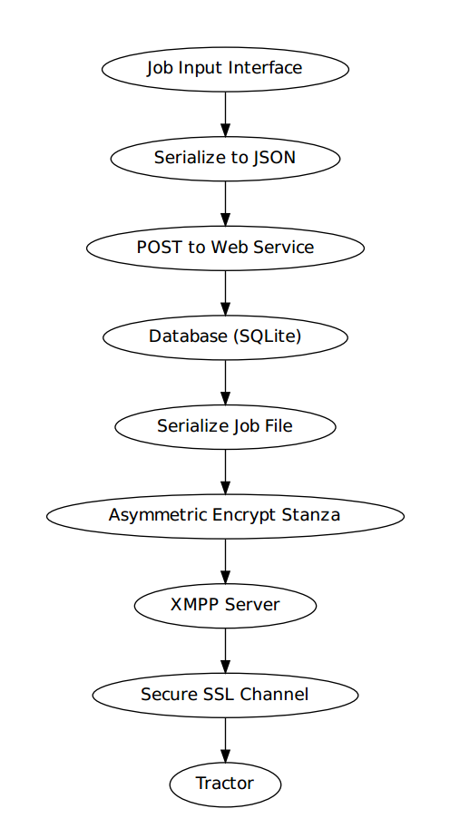
\includegraphics[width=0.4\textwidth]{Images/signalpath.png}
\caption{\DIFaddFL{High Level Signal Path}}
\label{fig:signalpath}
\end{figure}

\DIFaddend \subsection{Task 1 : Development Environment}
This task consisted of setting up the development environment for the
RoboTractor project. A project homepage was provided to us via the ASU virtual
lab project. This home page provides source control in the form of a GIT
repository which our project takes advantage of. \DIFaddbegin \DIFadd{In addition we used the amazon's cloud service to develop and test our project. }\DIFaddend Additionally, two virtual machines were provided via the ASU virtual lab project to use as our project servers. Setup of these servers was automated with the creation of a script in order to download all required software packages. Remaining work for this task is to enable proper connectivity between the two assigned Virtual Machines.
\DIFdelbegin %DIFDELCMD < 

%DIFDELCMD < %%%
\DIFdel{RoboTractor on built on the Django }\DIFdelend \DIFaddbegin \DIFadd{RoboTractor is built upon the Django Web Framework}\DIFaddend . The development environment is best
described in \autocite{_django_2014}. The Development environment consists of
\DIFdelbegin \DIFdel{2 Fabric configurations}\DIFdelend \DIFaddbegin \DIFadd{two fabric configurations: }\DIFaddend one for development and a second for deployment. This
allows development settings to be more relaxed facilitating quick coding
cycles, while the deployed configuration is more secure. Separate database
also prevent test data from polluting the deployed demo project.

\subsection{Task 2: XMPP Implementation}
\label{sec:xmpp}
XMPP \DIFdelbegin \DIFdel{Implementation is a configuration task to setup the ejabberd server and
connect it into the HTTP Framework. The XMPP client/server components and
interfacing with them is not a midterm deliverable, and is to be finished before
final submission.
}%DIFDELCMD < 

%DIFDELCMD < %%%
\DIFdel{XMPP }\DIFdelend provides an SSL/TLS connection between the tractor, and the server. This
allows a base level of secure communication.  However to augment the security
model, we provide \DIFaddbegin \DIFadd{an }\DIFaddend additional asymmetric encryption of the command structures
in each XMPP stanza. This \DIFaddbegin \DIFadd{project }\DIFaddend also leverages a Trusted Platform
Module (TMP). TMP is a hardware module, either part of the compute engine
complex or as in ARM processors integrated into the CPU core itself.  ARM's
offering is called TrustZone.  These security services provide a hardened
storage location for private keys.  One cannot extract the key without
destroying the device, and the key itself.  These devices also leverage a best
practice called \DIFdelbegin \DIFdel{``}\DIFdelend \DIFaddbegin \DIFadd{"}\DIFaddend Root of Trust\DIFdelbegin \DIFdel{'' }\DIFdelend \DIFaddbegin \DIFadd{" }\DIFaddend to protect against known cipher attacks\DIFaddbegin \DIFadd{.
}\DIFaddend \autocite{_tpm_2013}.  The hardware modules only decrypt/encrypt material if the system is in a \DIFdelbegin \DIFdel{``secure''
}\DIFdelend \DIFaddbegin \DIFadd{"secure" }\DIFaddend state.  Typically this is obtained by the compute core booting an internal,
untamperable ROM loader.  This loaders verifies the second stage bootloader with
a cryptographic signature stored in the TPM device at production time. If this
signature passes, the TPM is unlocked and the hardware may continue booting. If
any signature fails, the TPM remains locked, and refused to cipher information.
For the purposes of RoboTractor this behavior will be simulated at the API
level.  However hardware integrators may leverage the best practices laid out
here to implement a \DIFdelbegin \DIFdel{``}\DIFdelend \DIFaddbegin \DIFadd{"}\DIFaddend root of trust\DIFdelbegin \DIFdel{'' }\DIFdelend \DIFaddbegin \DIFadd{" }\DIFaddend to include the automation server. \DIFaddbegin \DIFadd{Specifically in RoboTractor, this TPM is simulated with an additional Python module entitled TPM.py. By having to include this module on both the server and client sides, the full TPM functionality is simulated. Without this module, the system will not be functional.
}\DIFaddend 

\subsection{Task 3: \DIFdelbegin \DIFdel{Demo }\DIFdelend \DIFaddbegin \DIFadd{Simulation }\DIFaddend Tractor \DIFaddbegin \DIFadd{Agent}\DIFaddend }

\begin{figure}
\centering
\DIFdelbeginFL %DIFDELCMD < 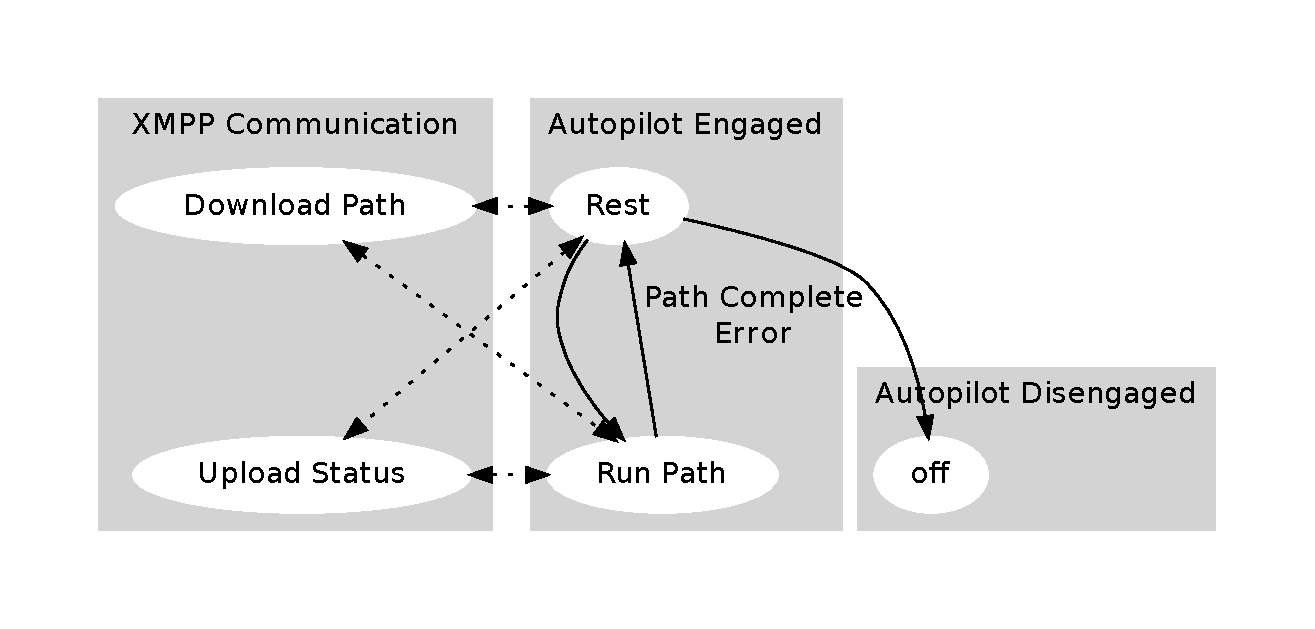
\includegraphics[width=0.4\textwidth]{machine.pdf}
%DIFDELCMD < %%%
\DIFdelendFL \DIFaddbeginFL 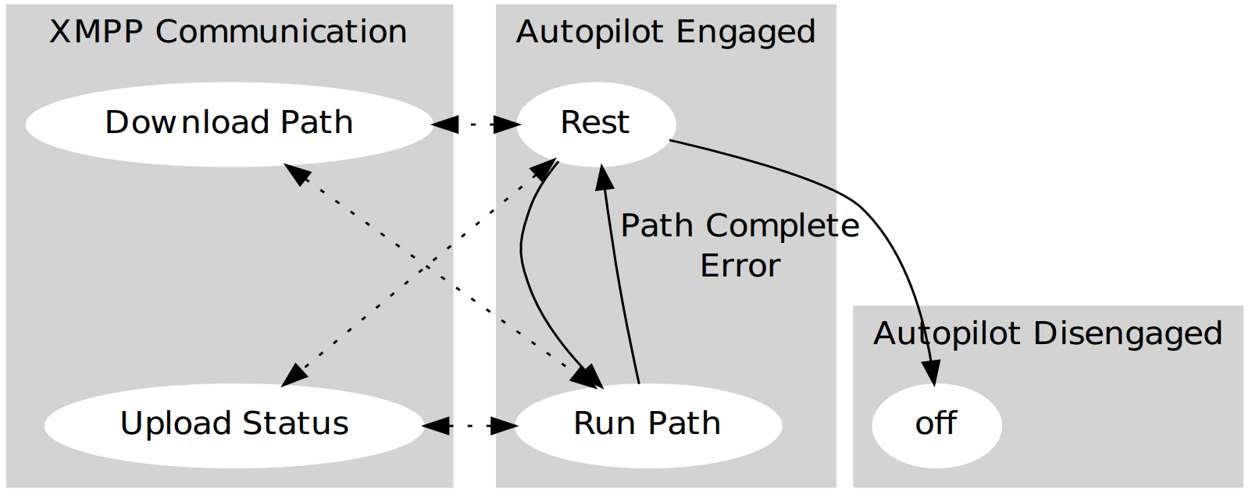
\includegraphics[width=0.4\textwidth]{Images/machine.png}
\DIFaddendFL \caption{Tractor Software State Machine}
\label{fig:tractorstatemachine}
\end{figure}
The \DIFdelbegin \DIFdel{midterm }\DIFdelend \DIFaddbegin \DIFadd{final }\DIFaddend deliverable for this task was to \DIFdelbegin \DIFdel{finalize the design specifications
of }\DIFdelend \DIFaddbegin \DIFadd{implement }\DIFaddend the tractor simulator. This
has been achieved after multiple team discussions, and a \DIFdelbegin \DIFdel{basic state machine vehicle simulator has been }\DIFdelend \DIFaddbegin \DIFadd{state machine based
vehicle simulator was }\DIFaddend written in python. \DIFdelbegin \DIFdel{As more tasks are completed, the simulator is to be updated with its
required functionality }\DIFdelend \DIFaddbegin \DIFadd{Tasks }\DIFaddend such as XMPP communication, path
processing, and status reporting \DIFaddbegin \DIFadd{were completed, and the simulator was updated
with its required functionality}\DIFaddend . The state machine consumes the Job File format
described in Figure~\DIFdelbegin \DIFdel{\ref{fig:jobfile}}\DIFdelend \DIFaddbegin \DIFadd{\ref{fig:job_file}. Additionally, the vehicle simulator
employs usage of public-key cryptography for its communications with the XMPP
server. This ensures that the control and signals between the two are secure and
provide high information assurance. Upon initial startup of the vehicle
simulator agent, a session-key request message is encrypted with the server's
public key. Once the server decrypts this request, it is processed, and
a session key encrypted with the agent's public key is sent back. The vehicle
simulator agent then decrypts the session key. This session key is used from
here on out to encrypt and decrypt communication data that is being sent as the
``body'' of an XMPP message. 
}

\DIFadd{Because the goal of the RoboTractor project is to for remote control and
signaling of an automated vehicle, mapping and coordinates play a big role in
the simulator's operation. As a result, much of the operation of the vehicle
simulation agent relies on mathematical formulas involving GPS coordinates.
Thorough testing of these algorithms and formulas had to be done to ensure that
the operation of RoboTractor was as intended. Current operation of the Vehicle
Simulation Tractor is as follows: Upon startup, the tractor enters a state in
which it queries the XMPP server to provide a session key
(Figure~\ref{fig:tractorstatemachine}). Once this session key
is securely established, the simulation agent sends an encrypted request for job
data. The XMPP Server interfaces with the database and front-end to build a JSON
object containing this data, encrypts it, and sends it to the simulation agent.
From here, the simulation agent processes the data to build its waypoints and
path, and begins its simulated 'movement'. After every tic of movement, the
agent sends an encrypted status update back to the XMPP server, which can then
update the Front-end for user visibility}\DIFaddend . 

\begin{figure}
\centering
\DIFdelbeginFL %DIFDELCMD < 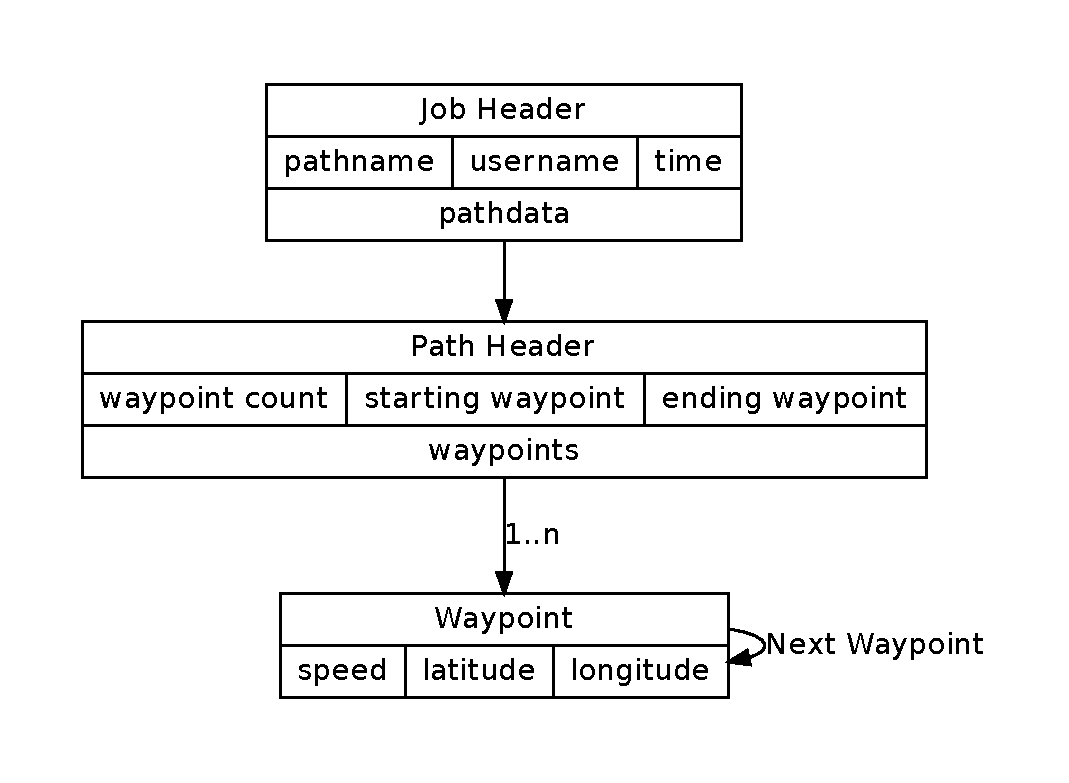
\includegraphics[width=0.4\textwidth]{job_file.pdf}
%DIFDELCMD < %%%
\DIFdelendFL \DIFaddbeginFL 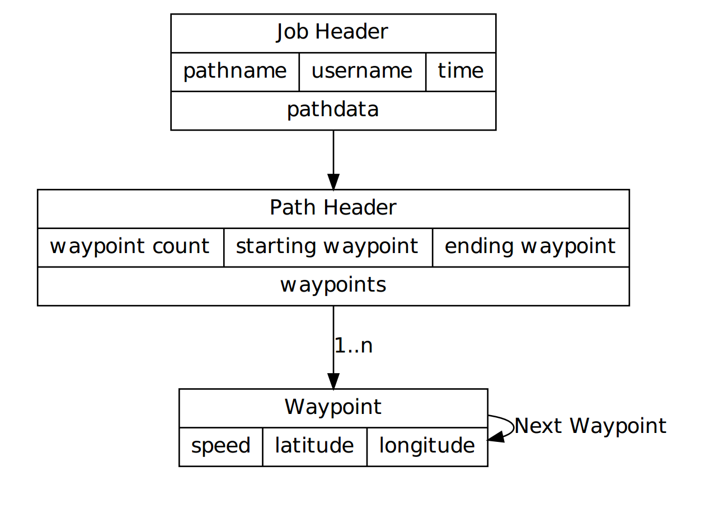
\includegraphics[width=0.4\textwidth]{Images/job_file.png}
\DIFaddendFL \caption{Job File Format}
\DIFdelbeginFL %DIFDELCMD < \label{fig:jobfile}
%DIFDELCMD < %%%
\DIFdelendFL \DIFaddbeginFL \label{fig:job_file}
\DIFaddendFL \end{figure}

As described in Figure~\ref{fig:signalpath}, the job files are stored in the
database. When the Tractor is instructed to run a job, the Tractor downloads the
Job file from the server over its \DIFaddbegin \DIFadd{secure }\DIFaddend XMPP connection. The backend server is
responsible for translating the database models into \DIFaddbegin \DIFadd{a }\DIFaddend JSON encoded Job\DIFaddbegin \DIFadd{. The tractor simulation agent decodes this JSON encoded job, and then processes its accompanying data fields as needed. Similarly, when sending status and waypoint data back to the server, it is first encoded as a JSON object, then encrypted, then sent. 
}\DIFaddend File \autocite{_json_2014}.

\subsection{Task 4: Frontend UI}
\begin{figure}
\centering
\DIFdelbeginFL %DIFDELCMD < \includegraphics[width=0.4\textwidth]{../PlottingV1.png}
%DIFDELCMD < %%%
\DIFdelendFL \DIFaddbeginFL \includegraphics[width=0.4\textwidth]{Images/PlottingV1.png}
\DIFaddendFL \caption{Job Input Tool}
\label{fig:jobinput}
\end{figure}

The \DIFdelbegin \DIFdel{"}\DIFdelend \DIFaddbegin \DIFadd{``}\DIFaddend single-page\DIFdelbegin \DIFdel{" }\DIFdelend \DIFaddbegin \DIFadd{'' }\DIFaddend web application is the modern design methodology to web
applications today. Leveraging this design architecture the \DIFdelbegin \DIFdel{Frontend will query }\DIFdelend \DIFaddbegin \DIFadd{front-end queries }\DIFaddend the REST API
to draw the position of all tractors within a Google Map context. Additionally, 
the frontend user interface is to be highly secure. \DIFaddbegin \DIFadd{Since the web frontend this provides a control
channel to functioning machinery, security directly correlates to the safety of
the system. }\DIFaddend This task has
\DIFdelbegin \DIFdel{2 }\DIFdelend \DIFaddbegin \DIFadd{three }\DIFaddend high level sub tasks:

\begin{enumerate}
\item Path \DIFdelbegin \DIFdel{generation
}\DIFdelend \DIFaddbegin \DIFadd{Design and Input
}\DIFaddend \item Map \DIFdelbegin \DIFdel{rendering
}\DIFdelend \DIFaddbegin \DIFadd{Rendering
}\DIFaddend \item Two-Factor Authentication
\DIFdelbegin %DIFDELCMD < \item %%%
\DIFdel{Vehicle location validation (final deliverable)
}\DIFdelend \end{enumerate}

\DIFdelbegin \DIFdel{Path generation is the primary deliverable of this task. The user shall be }\DIFdelend \DIFaddbegin \DIFadd{Via the web interface the user is }\DIFaddend able to input a path for a given tractor to
drive \DIFaddbegin \DIFadd{(Figure~\ref{fig:jobinput})}\DIFaddend . Our map
rendering system allows the user to select the waypoints just by clicking on the
map for which the system returns the latitude and longitude location information
to the \DIFdelbegin \DIFdel{user}\DIFdelend \DIFaddbegin \DIFadd{REST interface, once successfully posted (HTTP 201), the UI renders the
respective point on the map}\DIFaddend . The user then can select that location as a waypoint, on top of
which the real-time markers will be placed to display location and waypoint
information. Through this method the user can select a number of waypoints and
generate the path for a tractor. The path generation algorithm generates the
path \DIFdelbegin \DIFdel{just }\DIFdelend by drawing a straight line between the waypoints in the order of the
waypoints selected by the user. The \DIFdelbegin \DIFdel{path generated is then overlayed }\DIFdelend \DIFaddbegin \DIFadd{generated path is then laid }\DIFaddend on top of
the rendered Google map. By this way the user can view the path on the real time
map. 
\DIFdelbegin \DIFdel{Waypoints
input by the user, and sent to the backend web-service via the REST interface.
}\DIFdelend \DIFaddbegin 

\DIFaddend The webservice stores the waypoints in a Model format until
instructed to convert it to the Job Format and send it to the Tractor.  \DIFdelbegin %DIFDELCMD < 

%DIFDELCMD < %%%
\DIFdel{The
Tractor will then receive }\DIFdelend \DIFaddbegin \DIFadd{The
Tractor receives }\DIFaddend this path over the XMPP channel \DIFaddbegin \DIFadd{through the
aforementioned secure communication channels}\DIFaddend . The UI periodically queries REST
endpoint for the \DIFdelbegin \DIFdel{current position of the tractor }\DIFdelend \DIFaddbegin \DIFadd{position updates since the last query, which the XMPP server writes
to a database after it receives position updates from the Vehicle simulation
agent, }\DIFaddend and updates it on the Google Map. 
\DIFdelbegin \DIFdel{The UI will also include automated two-point
vehicle location validation, where the location of the vehicle is checked
against the boundary. Currently, a test-interface has been completed to meet the midterm deliverables, with additional functionalityforthcoming}\DIFdelend \DIFaddbegin \DIFadd{Additionally, robotractor has a real-time path view
functionality where the farmer/owner can view the agricultural vehicle status in
real-time. The vehicle is designed to report its location every five seconds.
The location of all the vehicles is updated to the database and then live view
functionality pulls the latitude and longitude location information from the
database and renders them on the Google map. This interface as shown in
Figure~\ref{fig:livejobpage}. This function also has security implications as
the location tracking can also mitigate vehicular theft. Since all the
communications are protected by a dual layer encryption, the transmissions cannot
be tampered with easily. Hence it is difficult for an attacker to perform
attacks on the system. 
}


\begin{figure}
\centering
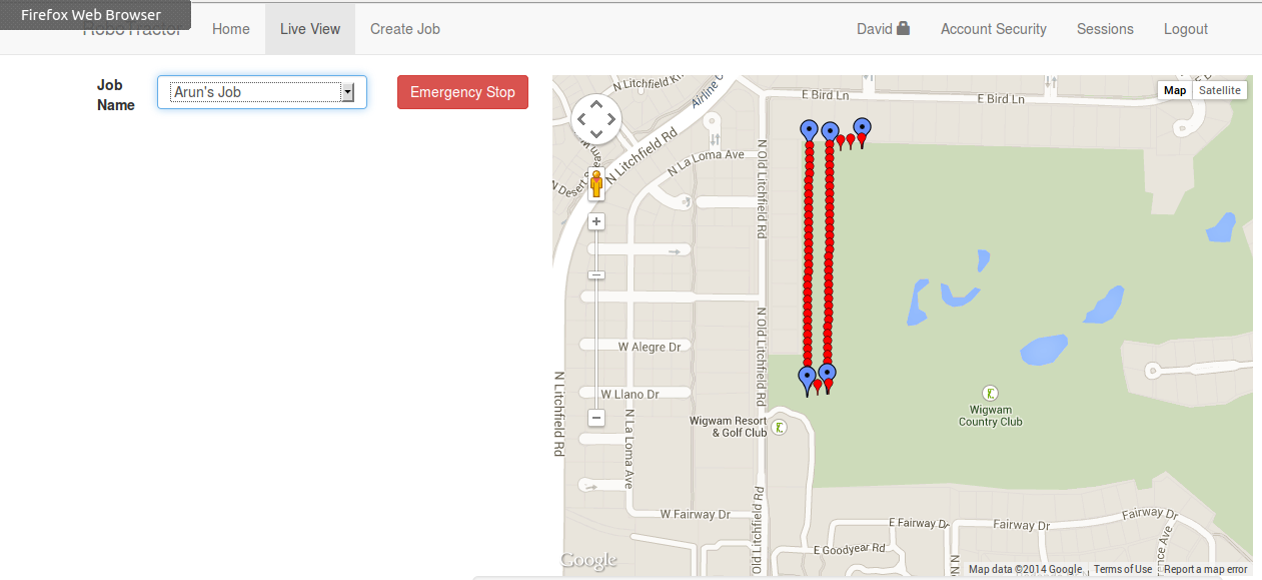
\includegraphics[width=0.5\textwidth]{Images/Picture6.png}
\caption{\DIFaddFL{Live Job View Page}}
\label{fig:livejobpage}
\end{figure}

\DIFadd{The RoboTractor also have schedule and boundary functionality, where the
farmer/owner can use the scheduler functionality to upload job to the database
without actually launching it, which can be done later. The Vehicle Location
Validation functionality allows the farmer/owner to set up the boundary of
his/her farm beyond which the vehicles will be either made in-operable or
disabled to mitigate the vehicular thefts or accidents. Within the Vehicle
Simulator designed this is as simple as moving the vehicle to the shutdown
state}\DIFaddend . 

\subsection{Task 5: Server Backend}
The Server Backend is the critical component which connects all \DIFdelbegin \DIFdel{components}\DIFdelend \DIFaddbegin \DIFadd{further
subsystems}\DIFaddend .
Extensive knowledge of Django will make this task easier. As it will require
linking multiple components together in a orchestrated fashion. \DIFaddbegin \DIFadd{Our initial
design used an existing Punjab library to connect Django to eJabberd
}\autocite{_twonds/punjab_2014}\DIFadd{. However once we began implementing the interface
we found since were were extending the XMPP session only to the REST interface
and not all the way to the web browser, the advanced functionality of Punjab was
unnecessary.  Instead we used SleekXMPP to setup the backend as an XMPP client.
All tractors in the system connect to this XMPP endpoint, and the server indexes
the Jabber ids against registered machines in the database. REST communicates to
the database. This backend service uses that database to communicate to clients. 
}

\DIFaddend We have
currently setup and tested our server running on Django\DIFdelbegin \DIFdel{, and will continue to
update as needed over the course of the project.
}%DIFDELCMD < 

%DIFDELCMD < %%%
\DIFdelend \DIFaddbegin \DIFadd{.
}\DIFaddend This task also includes the Service Side Session-Based Authentication. The
Server is responsible for generating the Time based One-Time Password (TOTP) as
described in RFC 6238 \autocite{rydell_totp_2011}. TOTP provides the ``thing you
have''
authentication factor. RFC 6238 describes generating a QR code from a private
seed value. This setups up the preshared key between the user and the web
service. At this point the user may use an standard authenticator app, such as
Microsoft Authenticator or Google Authenticator. At each sign on, the user is
prompted for their password ``the thing you know'', as well as a random number
from their device, \DIFdelbegin \DIFdel{``}\DIFdelend \DIFaddbegin \DIFadd{"}\DIFaddend the thing you have\DIFdelbegin \DIFdel{''}\DIFdelend \DIFaddbegin \DIFadd{"}\DIFaddend .  Additionally, this helps prevent
replay sign-on attacks since the transaction requires knowledge of the
\DIFdelbegin \DIFdel{preshared }\DIFdelend \DIFaddbegin \DIFadd{pre-shared }\DIFaddend key to generate the unique sign on credentials.
\DIFdelbegin \DIFdel{The midterm
presentation provides a video demo of this functionality.
}\DIFdelend 

\subsection{Task 6: REST Interface}
The REST interface \DIFdelbegin \DIFdel{will server }\DIFdelend \DIFaddbegin \DIFadd{serves }\DIFaddend the primary means of interacting with the \DIFdelbegin \DIFdel{site}\DIFdelend \DIFaddbegin \DIFadd{system}\DIFaddend .
The Web interface \DIFdelbegin \DIFdel{will exist as a "}\DIFdelend \DIFaddbegin \DIFadd{exists as a ``}\DIFaddend single-page\DIFdelbegin \DIFdel{" app }\DIFdelend \DIFaddbegin \DIFadd{'' application }\DIFaddend which leverages AJAX
principles over this REST API. The REST interface is currently functional, and
will be updated to interface further with the frontend interface and backend
components as they are completed.

The REST API is self documenting in the JSON format. Each endpoint publishes the
data, as well as its supported services on the \texttt{/schema?format=json}
endpoints. While this provides API developers a straightforward way to view the
supported data, and required formats, being in JSON, a developer can also
dynamically discover the API and generate a site against it.  This is a common
idiom in enterprise web applications using dependency injection.  RoboTractor
supports this idiom over REST for more advanced use cases.

Lastly, since the REST interface is a command interface to actual machines, it
is critical that all requests are authenticated. The REST interface requires all
queries to come from two-factor authenticated sessions (as managed by the
backend service).  Each transaction contains a secured Cross-Site Forgery
Request Token, and all transport is secured by SSL. This is in line with best
practices for web services \autocite{ibm_best_2002}.

\subsection{Project Task Allocation}

From the tasks outlined in Section~\ref{sec:proj_desc}, the breakdown of work is
as follows: Jeremy Wright has configured the development environments and
\DIFdelbegin \DIFdel{the REST
Interface. Jeremy is also
looking into modelling }\DIFdelend \DIFaddbegin \DIFadd{configuration and development of the REST and Frontend interface. Jeremy also
researched into modeling }\DIFaddend trust zones which \DIFdelbegin \DIFdel{would }\DIFdelend allow us to simulate trusted hardware
in actual vehicles.  He \DIFdelbegin \DIFdel{is operating }\DIFdelend \DIFaddbegin \DIFadd{operated }\DIFaddend as the project lead due to his experience in
Python-based Web Applications.  Arun Balaji Buduru \DIFdelbegin \DIFdel{is working }\DIFdelend \DIFaddbegin \DIFadd{worked }\DIFaddend on the Server Backend
and Frontend UI components\DIFdelbegin \DIFdel{. He
has completed a front-end test interface
and is continuing to update it to
achieve all required functionality}\DIFdelend \DIFaddbegin \DIFadd{, specifically with regards to the mapping interface
and google maps API}\DIFaddend . David Lucero \DIFdelbegin \DIFdel{is working }\DIFdelend \DIFaddbegin \DIFadd{worked }\DIFaddend primarily on the Tractor simulation
agents and \DIFdelbegin \DIFdel{also XMPP implementation. A barebones tractor
simulation has been completed and will be continuously updated as the project
progresses}\DIFdelend \DIFaddbegin \DIFadd{their XMPP implementation, as well as assisting Jeremy in interfacing
components together}\DIFaddend . Each group member has approximately 30\% workload of the
project with the remaining 10\% shared due to the interconnected nature of all
components. A detailed task breakdown can be seen in the attached Timeline.

\subsection{Deliverables}

Midterm Deliverables:
\begin{enumerate}
\item Functioning REST Interface (completed)
\item Front-end Test Interface (completed, with additional two factor-authentication)
\item API documentation for using the REST interface as an external service. (completed)
\item API documentation for using the XMPP interface to act as a vehicle. (moved to final deliverable)
\item Finalized Design of Vehicle simulator (completed, with additional python test implementation)
\item Interim Progress Report (completed)
\item Updated Project Schedule (completed)
\item Interim Project PowerPoint Presentation (completed)
\end{enumerate}

Final Deliverables:
\begin{enumerate}
\item \DIFdelbegin \DIFdel{Finalized back-end server configuration including easy installation script(s)
}%DIFDELCMD < \item %%%
\DIFdelend Completed, secure front-end interface including two-factor auth and
    SSL/TLS (complete)
\item Vehicle Simulator with working component interfaces \DIFdelbegin \DIFdel{and simulated trust zone functionality
}\DIFdelend \DIFaddbegin \DIFadd{(complete)
}\item \DIFadd{Simulated Trust Zone Functionality (complete)
}\item \DIFadd{Asymmetric XMPP message encryption (complete)
}\DIFaddend \item Final Project Report \DIFaddbegin \DIFadd{(complete)
}\DIFaddend \item Final Project PowerPoint Presentation \DIFdelbegin %DIFDELCMD < \item %%%
\DIFdel{User-guide covering front-end interface, and including API documentation for REST and XMPP interfaces 
}\DIFdelend \DIFaddbegin \DIFadd{(complete)
}\DIFaddend \end{enumerate}

\subsection{Project Timeline}
The attached project timeline (generated from Microsoft Project) describes the
overall tasks of the project.

\section{Risk Management of the project}
Several potential issues have been identified that may pose risk to successful
completion of this project. These risks have been identified in Table
\ref{tab:riskmanagement}. Along with the description, ratings have been assigned
to each risk identified, and potential mitigation strategies are described\DIFaddbegin \DIFadd{. During the course of project development, each of these risks was taken into consideration. For the risk of connections between components, the mitigation strategy was to include security on component connections. In the final version of the RoboTractor project this is done in two ways. The first way is that the XMPP server/client connections use SSL/TLS by default. This means that their communication channel is secured. In addition, the actual messages passed between the simulator and the tractor are themselves encrypted, providing an additional level of advanced security on the communication channel. 
}

\DIFadd{Another risk identified was the correctness of the vehicle simulation agents. The mitigation strategy of this risk was to fully design the simulation agents first, before development, and to review and test the design to ensure it would meet all requirements. This strategy was carried out, and the vehicle simulation agent itself is highly extensible. This allows easy changes and modifications if needed, while maintaining functionality and security. 
}

\DIFadd{The third risk identified was improper configuration of components, which could lead to entire system functionality breaking down. The mitigation strategy identified for this risk was to thoroughly review and test components before, during, and after development. This strategy was carried out, by repeatedly testing the components as they were begin developed, with actual geographic waypoint data that the system would use if run in real life. Using this actual data also allowed us to verify the the algorithms and formulas used were operating correctly.
}

\DIFadd{The fourth risk identified was that of using incorrectly implementing PKI or configuring it incorrectly. This is a common risk, and is hard to detect. Our mitigation strategy was to keep it simple and follow best practices and methodologies. To accomplish this, we limited the cryptographic use in RoboTractor to only what was needed, and used standardized algorithms implemented with a widely accepted library (Pycrypto). 
}

\DIFadd{The last risk identified was that of Service uptime and web reliability. Because the RoboTractor project is web-based, this is very important. If the project is down, this means a farmer or vehicle operator would be unable to operate their machinery remotely. Our mitigation strategy for this risk was redundancy, and using cloud hosting to alleviate hardware reliance. This risk did actually make itself present during RoboTractor development, as the server and code repository we had requested through the ASU cloud system repeatedly went down. Instead, we used a secondary cloud hosting solution temporarily so that development and testing would not be hampered}\DIFaddend . 

\section{Conclusion}
This work continues to explore how REST and XMPP can help alleviate the growing
cost issues in Agriculture. By providing a base set of secure services future
integrators can extend the provided data services over this base framework.
Using the RoboTractor framework accelerates development by allowing content
providers to provide secure, integrity, and authentication to their own
agricultural focused service. 

Agricultural machines themselves are growing in complexity, and the number of ECUs,
integrated sensors, advanced engine management, government oversight
documentation, prescription maps, real-time agronomy, crop consulting, genetic
seeding, the list is unbounded. These services can all be accelerated, reduced
cost, and increased quality and timeliness with the addition of secure
connectivity. RoboTractor provides the framework for these content provides to
provide such services. It's an exciting time to see where growers are
incorporating technology to bring us our daily bread.

\printbibliography
\clearpage
\begin{landscape}
\begin{table}%[!t]
%\renewcommand{\arraystretch}{1.3}
\caption{Risk Management}
\label{tab:riskmanagement}
\centering
\begin{tabular}{c||c||p{2in}||p{2in}}
\hline
\bfseries Risk Description & \bfseries Risk of Failure & \bfseries Consequence of Failure & \bfseries Mitigation Strategy\\
\hline\hline
Connections between components must be secure
& Low
& Product would still function, but would lack security – information assurance will suffer
& Plan to include security on component connections ahead of time. Follow best practices (SSL/TLS)\\
\hline
Evaluation of Project depends on proper vehicle agents
& Medium
& System is unable to be tested if vehicle agents are inoperable or incorrect
& Vehicle agents will be designed first to ensure compatibility with all other components. Thorough review and testing of component to ensure proper functionality\\
\hline
Improper configuration of components
& Medium
& Components do not communicate properly with each other. System functionality is void
& Thorough reviews and testing of components to ensure proper functionality and communication\\
\hline
Incorrect PKI implementation and/or configuration
& Medium
& Puts all identified security domains at risk. PKI used becomes useless. System becomes vulnerable to outside attacks i.e. MITM
& Follow best practices and standards. No re-invention of the wheel\\
\hline
Service Uptime (web reliably)
& High
& Product is unusable if network connections are not operable
& Redundancy. Cloud hosting to alleviate hardware reliance\\
\hline
\end{tabular}
\end{table}
\end{landscape}
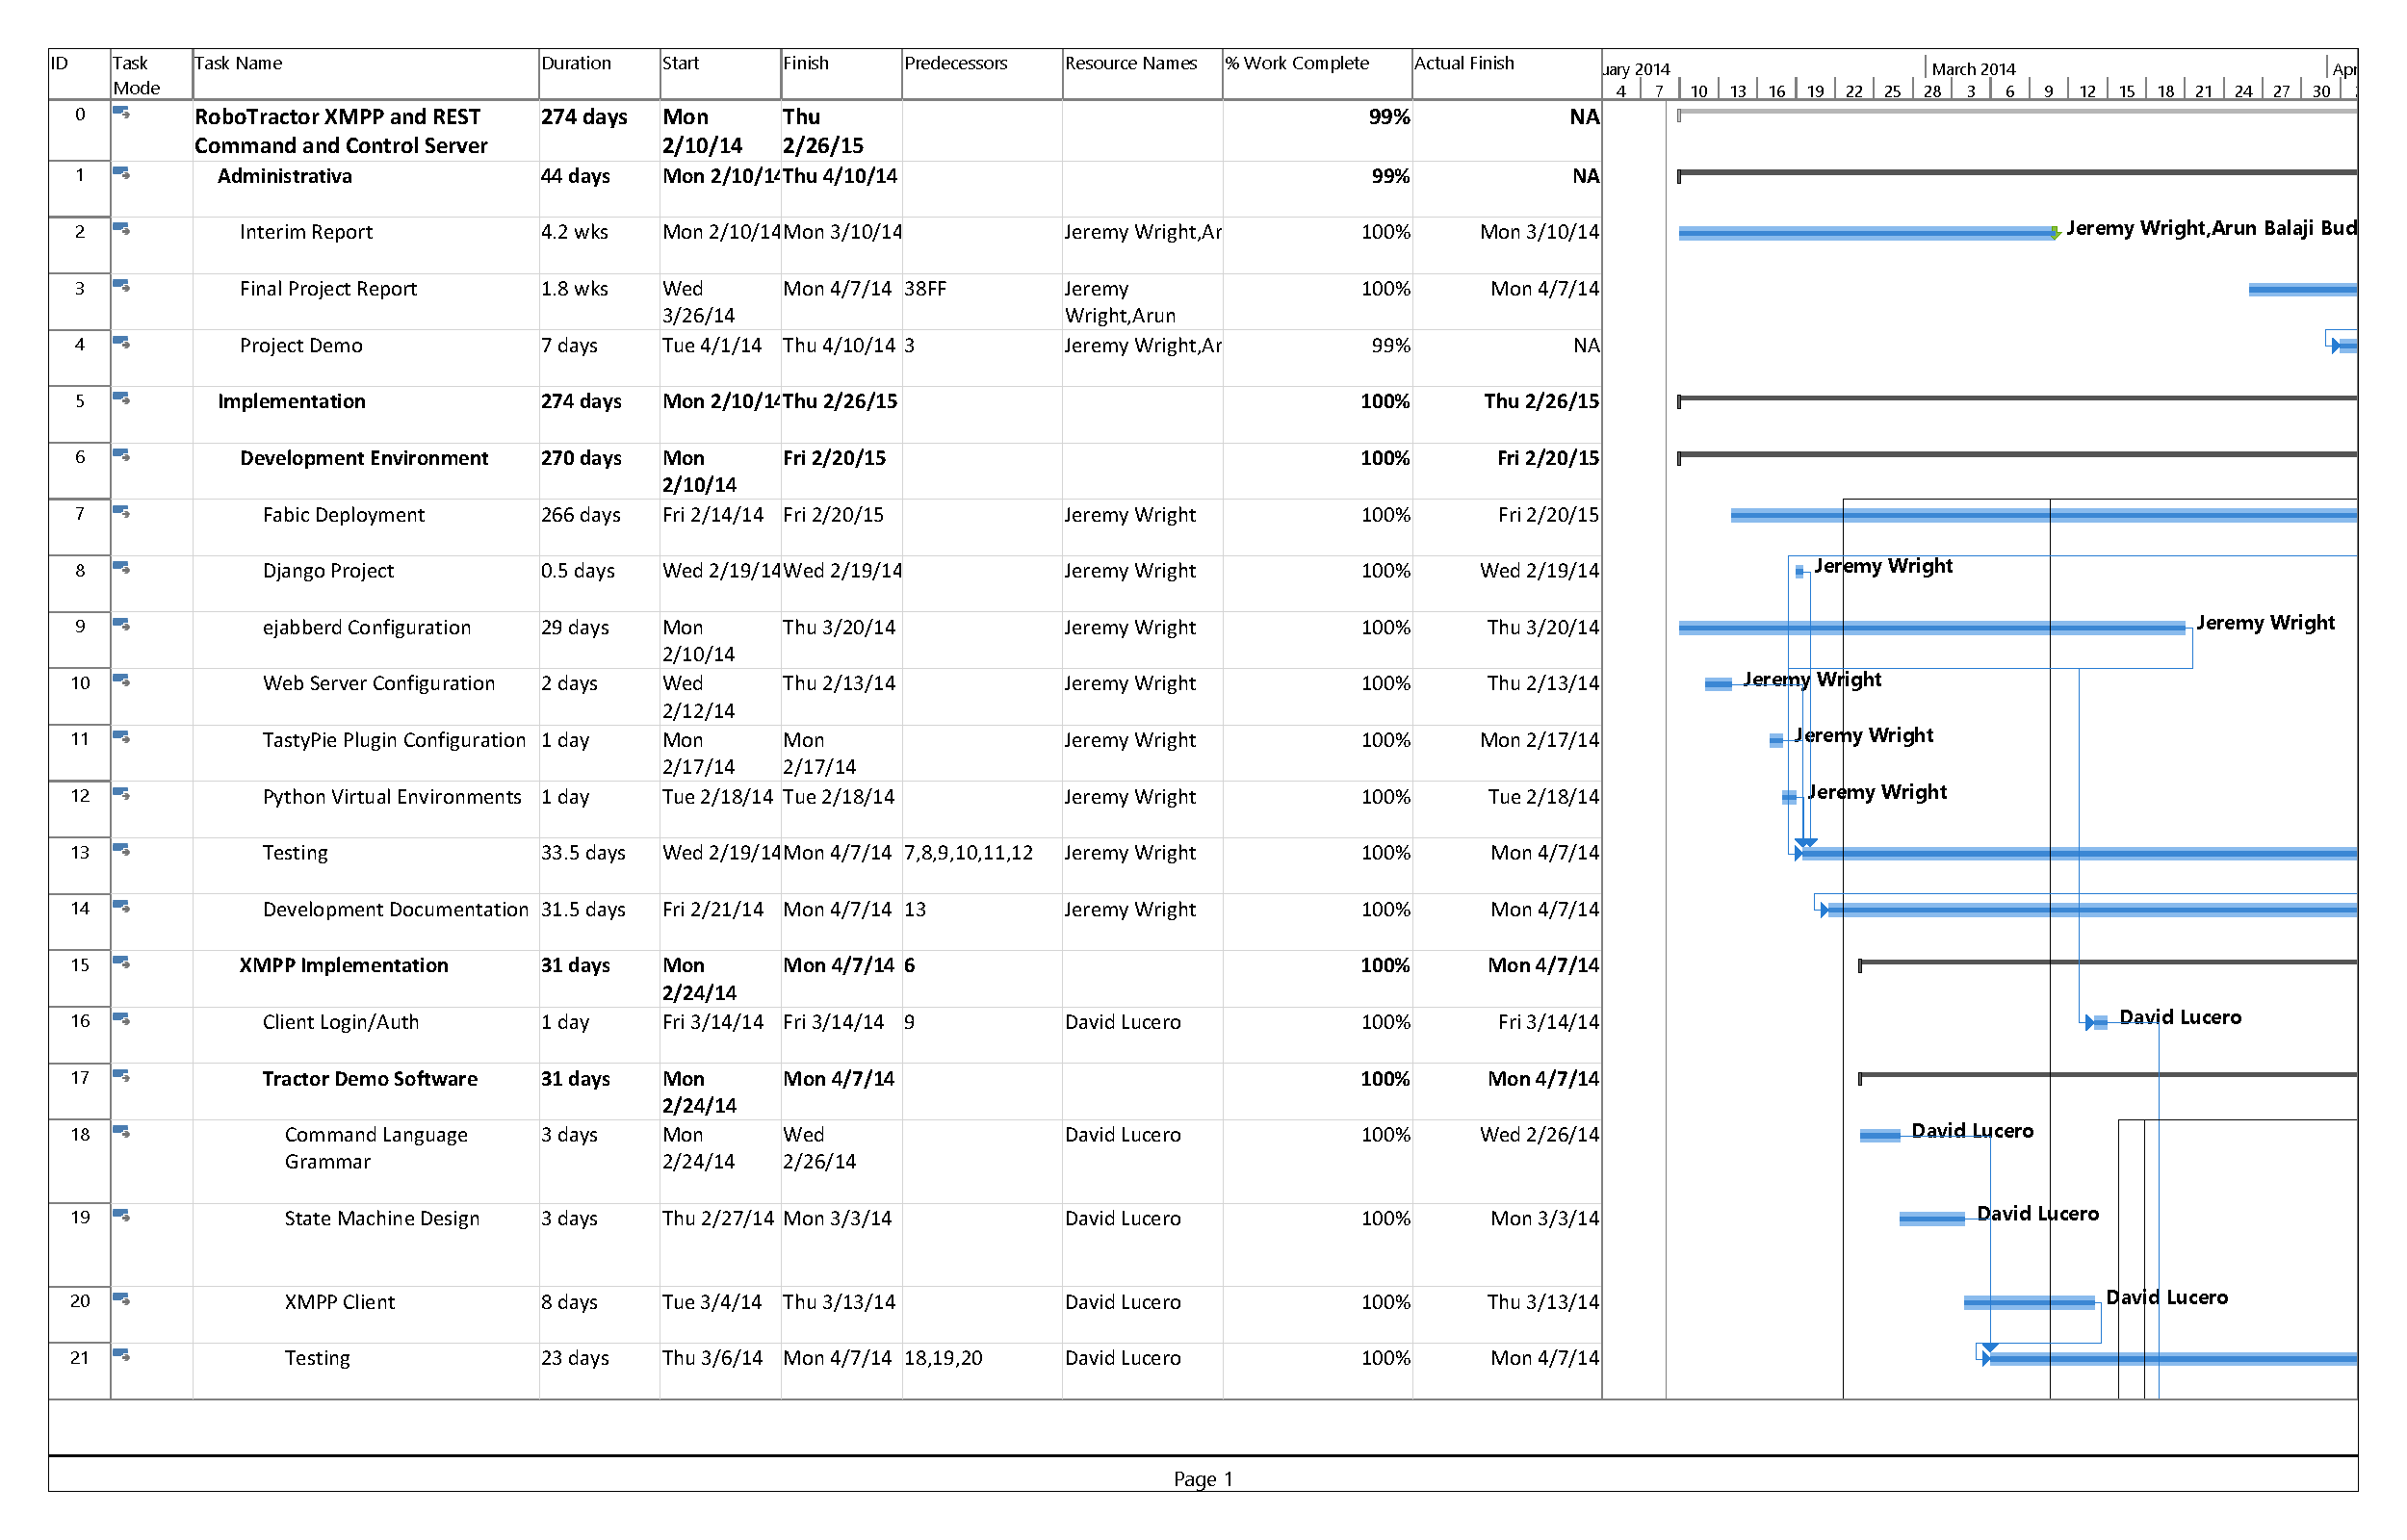
\includepdf[pages=-,landscape=true]{schedule.pdf}
\end{document}


